%!TEX root = ../main_text.tex
\chapter{Referencial Teórico} \label{chap:revisao_bibliografica}

Neste capítulo será descrito os principais conceitos necessários para o entendimento base dos fundamentos do trabalho, além de suas tecnologias e metodologias.

\section{Unidade de Processamento Central para \Wearables}
   Existem inúmeros tipos de processadores específicos para sistemas embutidos.
   A classe de processadores mais baratos e de baixo gasto energético usufruem de arquitetura geralmente de 8, 16 ou 32 bits na qual podem executar centenas de milhões de instruções por segundo.
   %
   Outra classe é na utilização de processadores de ponta, na qual são integrados a videogames ou \textit{switches} de rede.
   São processadores que possuem um custo elevado e executam uma taxa de bilhões de instruções por segundo, em comparação com o anterior.
   %

   Segundo \citet{Hennessy2011}, por mais que exista um leque de processadores para sistemas embutidos, o preço é um dos fatores mais importantes para a \design\ de um projeto, sendo tão importante quanto o requisito de desempenho pois necessita-se de um desempenho elevado a um preço reduzido.

   Tais processadores possuem o fim de serem aptos a cumprir os requisitos de uma aplicação \wearable\ como por exemplo o requisito de tempo real, na qual um segmento da aplicação possui um tempo de conclusão máximo absoluto.
   Outras situações também são permitidas, por exemplo um caso mais sutil na qual permite-se um tempo médio de restrição ao invés de um valor fixo, chamada de tempo real flexível.

   Com o uso de sistemas processados, a aplicação é executada totalmente em nível de \software\ por meio de instruções. Ou seja, ela é construída/compilada e executada diretamente pelo processador ou por um sistema operacional que intermedeia a aplicação com o seu fim, não usufruindo de nenhum aprimoramento oriundo de aceleradores em \hardware.
   %
   Além disso, todo este conjunto de sistema deve-se ser planejado junto com a quantidade de memória disponível para uso no \wearable\ pois, sabe-se que, quanto maior os recursos de memória, maior o seu gasto energético.



\section{\textit{Field-Programmable Logic Device} (FPGA)}
	% uso de fpga no mundo
	Até recentemente, os \hardwares\ reconfiguráveis eram utilizados unicamente na protitipação de projetos de circuitos integrados de aplicação especifica (ASIC, do inglês \textit{application-specific integrated circuit} e produção em baixo volume por causa de sua baixa velocidade e custo por unidade.
	Entretanto, com a variedade desses dispositivos disponibilizados hoje no mercado, em conjunto com a elevação do custo de engenharia não recorrente (NRE, do inglês \textit{Nonrecurring Engineering}, que refere-se ao custo de pesquisa, \design, desenvolvimento e teste de um novo produto e exigências de mercado), houve um crescente interesse na utilização de FPGAs para sistemas embutidos devido suas vantagens sobre ASICs em termos de flexibilidade de projeto e custo zero de engenharia não recorrente citada \citep{Mei2000}.
	%lousa branca
	Tais dispositivos, juntos com sua plataforma de interação, de forma geral, permitem ao \designer\ de sistemas embutidos ter uma \textit{lousa branca} em que possa implementar \hardwares\ computacionais personalizados tão facilmente como o desenvolvimento de um \software, como foi possível ilustrar na Figura \ref{fig:rt-board}.

	% Plataforma FPGA
	Dessa forma, uma \textit{plataforma FPGA} é um chip na qual, além de conter o componente FPGA, este está integrado à inúmeras interfaces e componentes, desde LEDs (do inglês \textit{Light-Emitting Diode}) e \textit{switchs} até porta Ethernet e interface vídeo VGA (do inglês \textit{Video Graphics Array}) e seus respectivos circuitos e como possui recursos suficientes para circuitos complexos, é possível implementar funções de processamento de imagem, interfaces de rede, algoritmos criptográficos e processadores completo, cada projeto de acordo com os recursos por ela disponibilizados. %\citep{Plessl2003}
	Entretanto, enquanto configurar um \hardware\ reconfigurável é uma tarefa fácil graças às ferramentas disponíveis hoje, criar um \design\ de \hardware\ inicial não é \citep{Sass2010}.

	\begin{figure}[h] \centering
		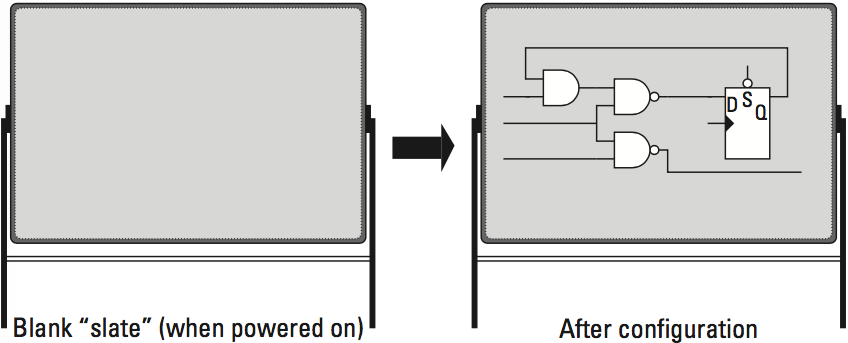
\includegraphics[width=0.75\textwidth]{img/rt-board.png}
		\caption{Ilustração em alto nível do funcionamento interno do FPGA. Fonte: \cite{Sass2010}.}
		\label{fig:rt-board}
	\end{figure}

	A seguir, será descrito a tecnologia que consiste os \hardwares\ reconfiguráveis, em especial o FPGA, e as respectivas linguagens de descrição de \hardware.

%\subsection{Sua Tecnologia}
   % PLD
   %Para introduzir alguns conceitos, é importante destacar o que são os dispositivos lógicos programáveis (PLDs, do inglês \textit{Programable Logic Devices}).
   %Às vezes chamados de dispositivos lógico programáveis em campo (FPLD, do inglês \textit{Field-Programmable Logic Device}), podem ser adaptados para criar muitos dispositivos digitais, desde simples portas lógicas até estruturas complexas.
   %\citet{tocci2003sistemas, Plessl2003} dizem que com um investimento de capital pequeno, qualquer empresa pode comprar os \softwares\ de desenvolvimento e \hardware\ necessário para programar PLDs para seus projetos digitais.
   %De modo geral, os PLDs são descritos como pertencendo a três tipo diferentes sendo eles os dispositivos lógicos programáveis simples (SPLD), dispositivos lógicos programáveis complexos (CPLDs, do inglês \textit{Complex Programmable Logic Devices}) e arranjo de portas programáveis em campo (FPGA) sendo o último tipo abordado neste trabalho \citep{Brown1996}.

   %LUTS
   O FPGA, item a ser utilizado nesta pesquisa, constitui de vários módulos lógicos programáveis relativamente pequenos e independentes, interconectados para criar funções maiores.
   Cada módulo lida, normalmente, com até quatro ou cinco variáveis de entrada.
   A maioria dos FPGAs utilizam uma \textit{look-up table} (LUT) para criar as funções lógicas desejadas.
   Uma LUT funciona como uma tabela-verdade, no sentido que a saída é programada para criar a função combinacional armazenando valores verdadeiros e falsos adequado a cada combinação de entrada.
   Os recursos de roteamento de sinal programável dentro do chip tendem a ser bem variados, com extensões de caminhos diferentes disponíveis.
   Os atrasos de sinal em um projeto dependem do roteamento real de sinal selecionado pelo \software\ de programação.
   Os módulos lógicos também contêm registradores programáveis.
   Eles não são associados a nenhum pino de entrada e saída (I/O, do inglês \textit{Input and Output}).
   Em vez disso, cada pino de I/O é conectado ao bloco programável de entrada e saída que, por sua vez, é conectado aos módulos lógicos com linhas de roteamento selecionadas.

   \begin{wrapfigure}{O}{0.5\textwidth} \centering
      \vspace{-10pt}
      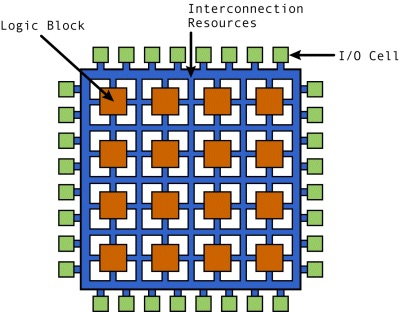
\includegraphics[width=0.5\textwidth]{img/rt-arch_fpga.jpg}
      \vspace{-15pt}
      \caption{Exemplo da arquitetura internas de um FPGA. Fonte: \url{http://www.eetimes.com/document.asp?doc_id=1274496}. Acesso: 30/05/2017.}
      \label{fig:rb-arch_fpga}
   \end{wrapfigure}

   Uma arquitetura geral simplista de FPGA é exibido na Figura~\ref{fig:rb-arch_fpga}. Nela os quadrados menores situado nas laterais são blocos de I/O que podem ser configurados para fornecer recursos de entrada, saída ou bidirecionais.
   Os quadrados maiores situados no interior são as LUTs, usados para guardar dados que entram ou saem e realizar as operações lógicas.
   Os canais que interligam os blocos entre si são estabelecidas por meio de conexões que passam pelas linhas e colunas nos canais entre esses blocos e possuem a funcionalidade de serem interconexões programáveis \citep{tocci2003sistemas}.
   %A tecnologia interna de um FPGA consiste basicamente de um arranjo de blocos lógicos, canais de roteamento para interconexão de blocos lógicos e blocos de entrada e saída de sinais em torno do circuito.
   %FPGAs baseado em SRAM (do inglês \textit{Static Random Access Memory}) utilizam células SRAM para controlar a funcionalidade de blocos lógicos e entrada e saída de sinais bem como as rotas, e pode ser reprogramado arbitrariamente em nível de circuito, muitas vezes, baixando um novo \textit{stream} de dados de configuração para o dispositivo.
   Hoje, esses dispositivos possuem milhões de portas de lógica programável, bilhões de transistores, além de outros blocos de \hardware\ dedicados dedicados como rápidas memórias embarcadas e multiplicadores de ponto-fixo tornando-o um dos circuitos integrados (CI) mais densos existente \citep{Choi2016}.

   \begin{comment}
   \begin{figure}[h] \centering
      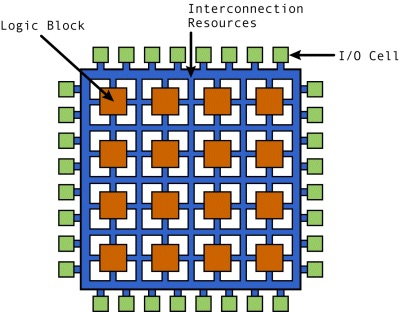
\includegraphics[width=0.5\textwidth]{img/rt-arch_fpga.jpg}
      \caption{Exemplo da arquitetura internas de um FPGA. Fonte: \url{http://www.eetimes.com/document.asp?doc_id=1274496}. Acesso: 30/05/2017.}
      \label{fig:rt-arch_fpga}
   \end{figure}
\end{comment}

   % tecnologia e energia
   Segundo \citeauthor{tocci2003sistemas}, tais maravilhas de flexibilidade de projetos digital podem fornecer uma série de opções de projeto sendo voltados para indústria e até mesmo educação.
   Ao utilizar tecnologia CMOS, o consumo de energia do chip é relativamente baixo comparado com outras tecnologias podendo ser confeccionado em nível de tensão elétrica, frequências e cargas para os sinais de I/O.
   O mercado fornece diferentes graus de velocidade de FPGA a fim de que o projetista utilize o mais adequado ao projeto.
   Entretanto, um dispositivo FPGA pode ser configurado para um número infinito de projetos e isso implica na não possibilidade de afirmar o montante de dissipação de energia para um dispositivo FPGA.
   %O \software\ Quartus II tem duas ferramentas para estimular o montante de uso de energia para uma aplicação.
   %O \textit{PowerPlay Early Power Estimator} é usado durante os estágios iniciais do projeto para estimar a magnitude de potência do dispositivo.
   Dessa forma, FPGAs são chips que podem ser programados instantaneamente para funções de qualquer circuito digital \citep{Choi2016}.

   % Importancia
   \citeauthor{tocci2003sistemas, Plessl2003} citam ainda que o motivo de PLDs estarem dominando o mercado é o fato de que, como são dispositivos programáveis, a mesma funcionalidade pode ser obtida com um circuito integrado (CI) ao invés de diversos circuitos individuais.
   Isso significa maior confiabilidade, menor espaço ocupado na placa, consumo de energia, complexidade de desenvolvimento e, geralmente, menor custo de fabricação.

   %\subsection{\textit{Hard} e \textit{Software Cores}}
   % Utilização de um processador sintético ou físico
   A unidade de processamento central (CPU, do inglês \textit{Central Processing Unit}) nesses tipos de sistema pode ser implementada em duas formas, sendo estas \textit{hard} e \textit{soft} \cores.
   O primeiro é um \core\ dedicado, ou seja, um pedaço de circuito integrado dentro (ou não) de um FPGA e o segundo é feito por meio da sintetização e mapeamento de um processador no FPGA com seus recursos lógicos, e assim, o processador é obtido por meio de \design\ e sintetização na placa por meio das portas lógicas.
   Independente da forma de projeto da CPU, o FPGA será constituído da seguinte arquitetura exibida na Figura~\ref{fig:rb-soc}, chamada de SoC FPGA (do inglês, \textit{System-on-Chip} FPGA).
   Nela, as setas representam os barramentos de comunicação entre os principais componentes.

   \begin{figure}[h] \centering
      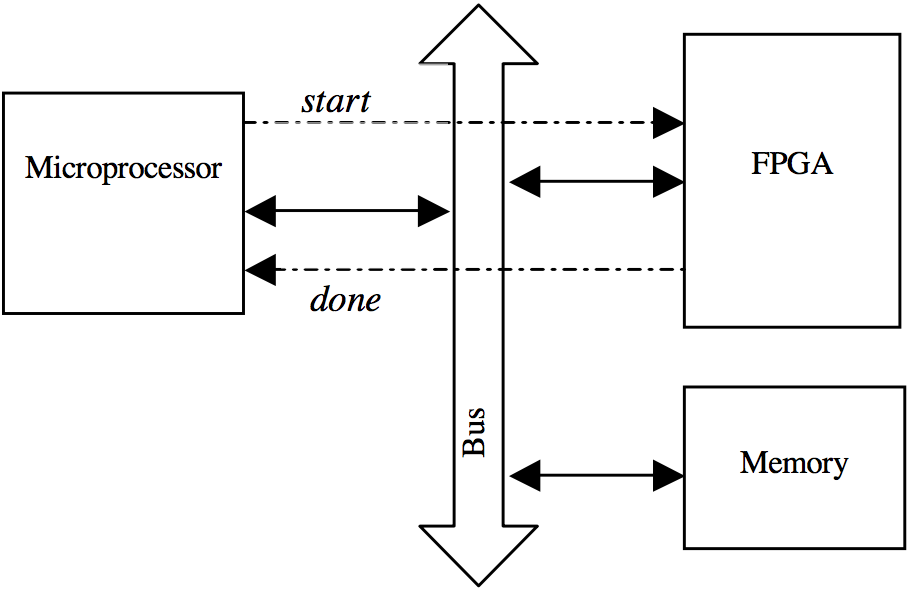
\includegraphics[width=0.6\textwidth]{img/into-soc.png}
      \caption{Visão geral de um SoC FPGA.}
      \label{fig:rb-soc}
   \end{figure}

   Cada um tipo de \core\ possui suas vantagens.
   Ao utilizar um \textit{hard} \core, é possível utilizar todos seus recursos obtendo máxima performance nas atividades executadas, a utilização de um \textit{soft} \core\ permite a extensão da arquitetura \citep{Plessl2003}.

   Um das maiores barreiras para o \design\ de projetos em FPGA é a necessidade de uso de linguagens de descrição de \hardware.
   Elas serão descritas a seguir.


	\subsection{\textit{Hardware Description Language} (HDL)}
		Linguagem de Descrição de \Hardware\ (do inglês \textit{Hardware Description Language}) é uma das classes de linguagens de computação usados para descrever formalmente um circuito eletrônico.
      Uma expressão padrão baseada em texto HDL é capaz de descrever o comportamento temporal ou a estrutura de circuito (espacial) de um sistema eletrônico.
      Sua origem veio da necessidade de documentar o comportamento do \hardware \citep{Sass2010}.

		HDL é amplamente utilizada em \design\ de \hardware\ especificando detalhes de \design\ de chip tantos chips específicos quantos os próprios FPGAs.
      Para customizar algum tipo de chip digital, HDLs especifica um modelo para um comportamento específico de um circuito antes do circuito ser projetado e construído.
      Ferramentas lógicas de sínteses são invocadas em seguida para gerar informações geométricas que são utilizadas para produzir as máscaras \textit{photolithographic}, necessárias para a fabricação do CI do projeto desenvolvido.

		A utilização de uma HDL é o primeiro passo no processo de síntese em FPGA.
      O código é entregue ao compilador lógico, chamado de ferramenta de síntese, e sua saída será carregada ao dispositivo reconfigurável.
		A propriedade única deste processo na qual fornece a lógica programável é que, com esse processo de síntese, é possível alterar o código HDL, compilá-lo e fazer sua síntese no mesmo dispositivo para testar, quantas vezes forem necessárias, sem custo adicional \citep{Smith1998}.

		Enquanto a maioria de engenheiros de \hardware\ utilizam tanto o \textit{VHDL} quanto o \textit{Verilog}, na qual possuem um nível elevado de complexidade \citep{Choi2016}, existe outras linguagens disponíveis para uso.
      Outras linguagens como \textit{SystemC}, \textit{HandelC} e \textit{Impulse} fornecem a construção de sistemas \hs\ juntos, dando ao \designer\ uma linguagem de alto nível para manuseio do projeto \citep{Sass2010}.


	\subsection{\textit{High-Level Synthesis} (HLS)}
		Sintetizador em Alto Nível (HLS, do inglês \textit{High-Level Synthesis}) são procedimentos que sintetizam códigos em alto nível para HDLs.

		Realizado uma especificação de \design\ em \software, um HLS pode reduzir os longos ciclos do processo de \design\ de \hardware\ e ainda trazer melhoria em performance e eficiência energética \citep{Choi2016}.

		As primeiras ferramentas sintetizadoras baseavam em linguagem \textit{C}, mas não houveram um sucesso em seu uso pois os engenheiros de \hardware\ acreditavam que existia uma lacuna entre o HLS e o \design\ de \hardware\ feito por humanos.
      A justificativa era que as ferramentas HLS não exploravam profundamente o recurso de paralelismo, além de que, para os engenheiros de \software\ HLS continua sendo uma dificuldade já que muitas partes do projeto, como a integração do sistema, permanecem em grande parte como um processo manual.

      Existem várias ferramentas para geração automática de código descritivo de \hardware.
      Ferramentas como o \textit{framework} LegUp e OpenCL \citep{Trevett2008} possuem o propósito de entregar um bom HLS além de tentar amenizar esses problemas de projetos.


      \subsubsection{LegUp High-Level Synthesis}
         LegUp é uma ferramenta que permite a utilização de técnicas de \software\ para implementação de \design\ de \hardware.
         Com o \textit{framework} LegUp, é possível utilizar um programa padrão  C como entrada e automaticamente compila o programa para dispositivos FPGA.

         É possível gerar procedimentos totalmente dispostos em \hardware\ e outros híbridos na qual é utiliza-se de \textit{soft} processadores, utilizando de um MIPS, e também gerando códigos para \textit{hard} processador que utiliza circuitos ARM disponibilizados em FPGAs SoCs pela Altera sendo tais gerações usufruindo de aceleradores que comunicam por meio de interface de barramentos padronizados \citep{Canis2011}.
         Possui também um \textit{framework} para \textit{debug} e verificação de HLS \citep{Fort2014}.

      \subsubsection{OpenCL}
         OpenCL é um padrão que oferece uma API comum para execução de programas em sistemas compostos por diferentes tipos de dispositivos computacionais tal como processadores \textit{multicores}, GPUs ou outros aceleradores.

         Este padrão utiliza de coprocessadores como meio para operações aritméticas intensivas paralelas e com isso é possível realizar realizar uma computação heterogênea paralela em nível de tarefas e dados, nos vários dispositivos disponíveis hoje pelo mercado criando um novo nível de infraestrutura computacional paralela.

         O OpenCL provê uma abstração fácil de uso e um amplo conjunto de APIs de programação baseada no sucesso obtido pelo CUDA (do inglês, \textit{Compute Unified Device Architecture}) e outros ferramentas de programação.
         Ele define um \core\ funcional que todos os dispositivos suportam incluindo uma mecanismo de extensão que permite os fabricantes exponham recursos de \hardware\ exclusivos e interfaces de programação experimentais para benefícios dos desenvolvedores de aplicações.

         De forma geral, um programa em OpenCL é executado num dispositivo computacional na qual os dispositivos podem conter um ou mais unidades computacionais (ou seja, \cores) na qual são compostas de um ou mais elementos de processamento SIMD (do inglês, \textit{single-instruction multiple-data}) \citep{Stone2010}.
         Como é possível visualizar na Figura \ref{fig:opencl}, levando para o ambiente de FPGAs, existe um \textit{host} que executa em um processador \textit{soft} ou \textit{hard} o \textit{ Runtime Environment} que fica responsável por controlar todos seus dispositivos.
         Cada dispositivo conectado ao \textit{host} pode conter vários \textit{processing elements} que por sua vez pode conter vários \textit{compute unit}.
         %De termos gerais, podemos associar com os conhecimentos de \software\ sendoos \textit{compute units} como \textit{threads}, \textit{processing elements} como \cores\ e os dispositivos como \textit{clusters}, sendo estes podendo ser heterogêneos.

         \begin{figure}[h] \centering
            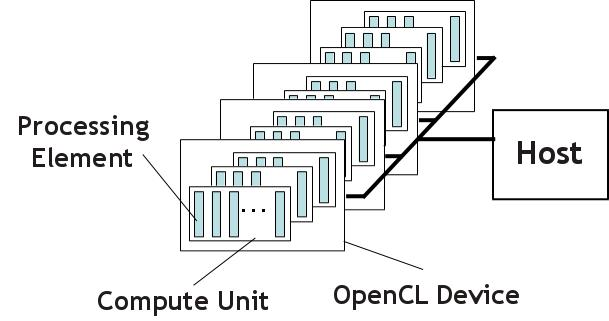
\includegraphics[width=0.7\textwidth]{img/opencl.jpg}
            \caption{Sistema hierárquico de um projeto em OpenCL. Fonte: \url{https://handsonopencl.github.io/} Acessado em: 07/08/2017.}
            \label{fig:opencl}
         \end{figure}

         Todos os aceleradores descritos neste relatório, podem ser associados com a sintetização dos procedimentos de instruções no FPGA \citep{Shagrithaya2013, Czajkowski2012}.

   		Para prover um melhor suporte para o paralelismo em \hardware, utilizaram de bibliotecas \textit{multi-threads} como a \textit{Pthread} \citep{Barney2009}, \textit{OpenMP} \citep{openmp} para criar aceleradores em \hardwares paralelos.

         É investigado otimizações em memória e arquitetura de sistema provendo melhorias em performance de circuito, área, utilizando uma abordagem do padrão produtor-consumidor para inferir circuito de transmissão em \hardware.

   \begin{comment}
   \section{Beagle Bone Black}
      Segundo \citet{Richardson2013}, além de um microcontrolador, o Beagle Bone Black é úm computador completo no qual possui suporte a sistemas como Linux Embarcado e Android, possuindo todos os componentes eletrônicos necessários para o seu funcionamento numa única placa impressa.
      Ao utilizar um sistema operacional embarcado, a placa torna-se hábil para suportar \textit{drivers} como periféricos USB e adaptadores podendo então ser adicionados módulos como câmera para captura de imagens e quaisquer outros adaptadores.

      Diferente de um típico microcontrolador que possem processadores de 8-bits, o Beagle Black Bone é capaz de compartilhar em seus processamentos em tarefas e programas, executados simultaneamente, criando um poder de processamento maior do que outros controladores sem o \textit{trade-off} do espaço\textit{die}.


      Este equipamento é voltado tanto para iniciantes com foco em aprendizagem no mundo de microcontroladores e sistemas embarcados, quanto usuários com conhecimentos avançados a fim de produzir produtos para fins mercadológicos.

      O autor \citet{Richardson2013} cita ainda que, ao comparar o Beagle Bone Black com o Raspberry Pi, o primeiro se destaca no fato de ser um produto com as características mais adequadas para fins profissionais, ou seja desenvolvimento de sistemas embarcados para projeto de produtos, o que não acontece nos dispositivos Raspberry Pi. Esses, por sua vez, possui o propósito de ser simples e didático, sendo seu \hardware\ e sistema voltados para tal.
\end{comment}


\section{\Profile} \label{sec:profile}
	%\begin{comment}
	%\end{comment}

		\Profile\ é uma procedimento para auxiliar o usuário a coletar informações do \software\ em tempo de execução.
      Existem vários programas diferentes para adquirir essas informações e podem ser distinguidos em duas categorias.
      A primeira é aqueles que apresentam a quantidade de declarações e invocações de rotinas, e aqueles que exibem informações de tempo de declarações e rotinas \citep{nemeth2004manual}. Um exemplo de saída é exibida a seguir.

{ \footnotesize
      \begin{verbatim}
Flat profile:

Each sample counts as 0.01 seconds.
  %   cumulative   self              self     total
 time   seconds   seconds    calls  ms/call  ms/call  name
 33.34      0.02     0.02     7208     0.00     0.00  open
 16.67      0.03     0.01      244     0.04     0.12  offtime
 16.67      0.04     0.01        8     1.25     1.25  memccpy
 16.67      0.05     0.01        7     1.43     1.43  write
 16.67      0.06     0.01                             mcount
  0.00      0.06     0.00      236     0.00     0.00  tzset
  0.00      0.06     0.00      192     0.00     0.00  tolower
  0.00      0.06     0.00       47     0.00     0.00  strlen
  0.00      0.06     0.00       45     0.00     0.00  strchr
      \end{verbatim}
      \vspace{-3em}
}

      \begin{wrapfigure}{o}{0.56\textwidth} \centering
         %\vspace{15pt}
         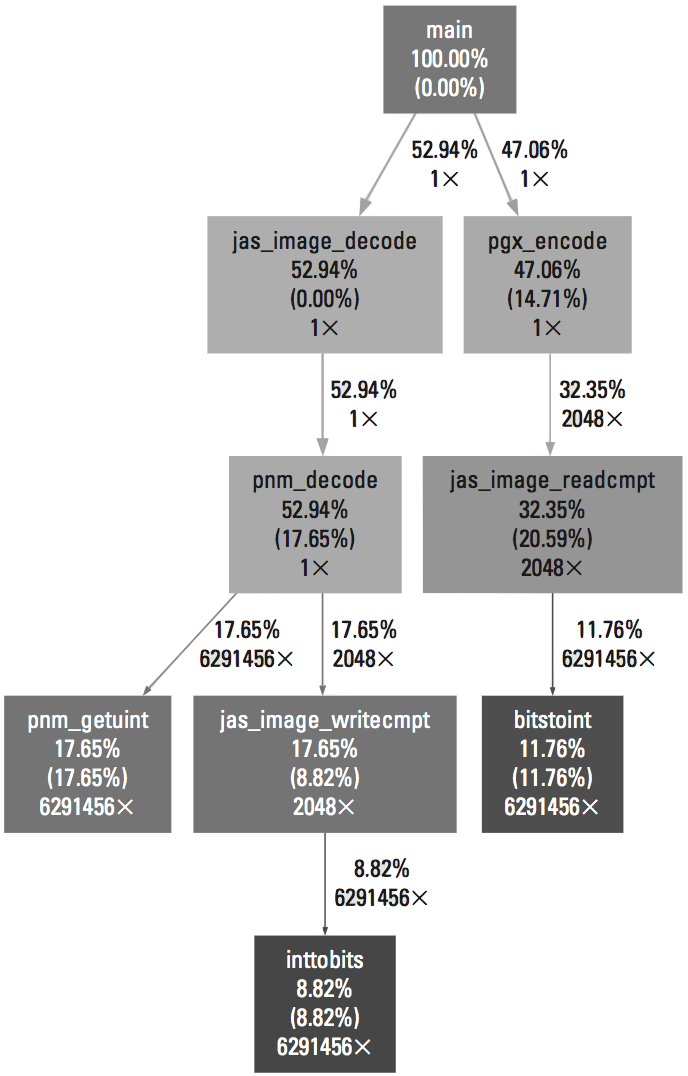
\includegraphics[width=0.48\textwidth]{img/f4-1-2.png}
         %\vspace{-1em}
         \caption{\Profile\ da codificação de imagem em formato JPEG. Fonte: \cite{Sass2010}. \vspace{-0em} }
         %\vspace{-3em}
         \label{fig:profile}
      \end{wrapfigure}

      A Figura \ref{fig:profile} exibe um exemplo gráfico de \profile\ de \software\ em um codificador de imagem em formato JPEG.
      O processo é feito ao colocar o \software\ referencial (programa a ser coletado) como entrada representativa na ferramenta e a coleta é realizada em várias partes da aplicação ao longo de sua execução neste.
		Uma das técnicas do \profile\ de mensurar uma aplicação é na realização de interrupções periódica no programa e amostrar o seu \textit{program counter}.
      Dessa forma, é possível utilizar um histograma para contar quando um programa é interrompido em um endereço particular e a partir dessa informação, calcular a fração aproximada do tempo total de execução gasto em suas partes.
      Distribuições GNU/Linux possuem a ferramenta \texttt{gprof} na qual avalia procedimentos enviados por parâmetro, realizando o cálculo de tais informações de \software\ \citep{Graham1982}.





\section{Sistemas Computacionais \Wearables}
	% Introdução histórica e geral
	Sistemas computacionais \wearables\ são sistemas que, com a possibilidade de ter um computador acoplado ao corpo, proporciona ao usuário um nível superior de informações contextualizadas dentro de um ambiente interativo \citep{Amorim2017}.

   Com a tecnologia digital constantemente melhorando à medida que a informação se torna sem-fio, os avanços demandaram mais fatores móveis e \wearable\ de produtos que possuem acesso à informação.
   Segundo \cite{Gemperle1998}, um produto que é \wearable, deveria ter sua `\textit{wearability}' sendo este definido como a interação entre o corpo humano e o objeto \textit{wearable} estendendo ao corpo em movimento.

	\begin{wrapfigure}{O}{0.5\textwidth} \centering
    	  \vspace{-10pt}
		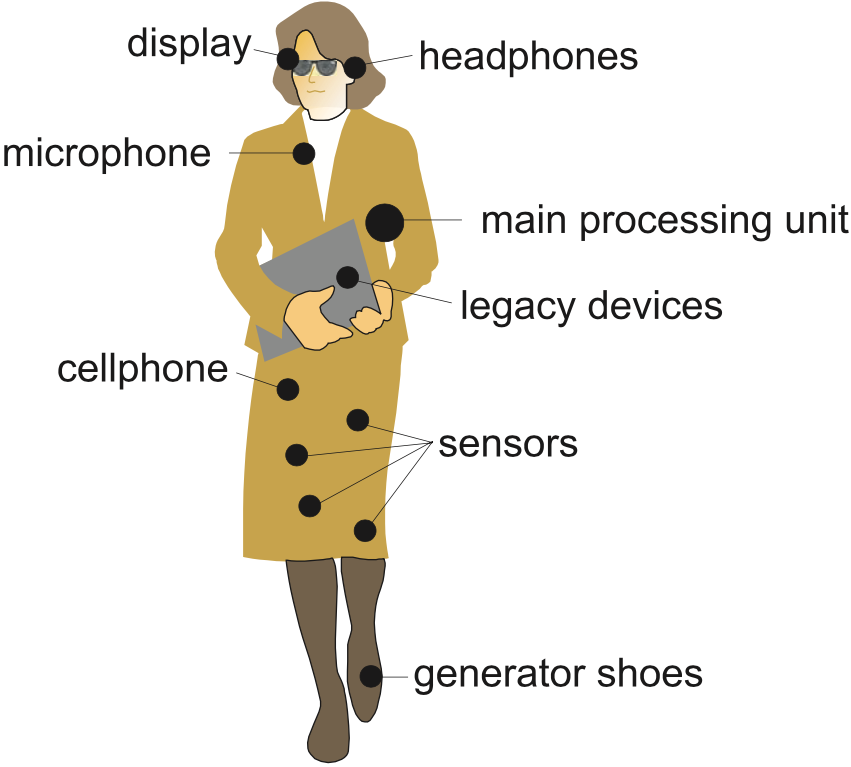
\includegraphics[width=0.5\textwidth]{img/into-wearable2.png}
        \vspace{-10pt}
		\caption{Exemplificação de alguns tipos de dispositivos \wearables. Fonte: \citet{Plessl2003}. \vspace{-15pt}}
		\label{fig:into-wearable}
	\end{wrapfigure}

	%\citep{Plessl2003}
	Devido ao movimento de seus usuários, um computador \wearable\ é embutido em um ambiente \mobile\ e necessita-se da interação com o ambiente ao seu redor.
	Como é exibido na Figura \ref{fig:into-wearable}, um sistema \wearable\ pode ser composto por um conjunto de nós distribuídos e uma rede de comunicação centralizada num módulo principal, sendo possível determinar, por exemplo, a geração de eletricidade por meio de geradores \textit{piezo-electric} integrados aos sapatos, energizando uma parte do sistema \wearable\ com o caminhar do usuário \citep{Kymissis1998} ou a ação do usuário por meio de acelerômetros \citep{VanLaerhoven2002, Kern2002}.

	Com a distribuição espacial dos módulos pelo corpo, a comunicação torna-se um item importante em termos consumo de energia \citep{Kymissis1998}.
   A rede de comunicação é uma mistura de conexões cabeadas e sem-fios.
   Para dispositivos \wearables, a comunicação sem-fio é a tecnologia predominante por causa da necessidade de mobilidade \citep{Plessl2003}.

	A introdução desses sistemas no ambiente de pesquisa não é nova como é reportado por \citet{Sutherland1968}, \citet{Mann1996} e \citet{Mann1997}.
   Entretanto, a aplicação desses dispositivos, depende diretamente da miniaturização dos componentes eletrônicos.
   Esse fenômeno fica claro ao perceber o crescente espaço ganho pelos \textit{smartwatches}, \textit{fitness trackers}, óculos, equipamentos de realidade virtual e aumentada e muitos outros nas indústrias e nas atividades pessoais de usuários.
   Com esses novos dispositivos embarcados de propósito geral miniaturizados, aumenta-se a sua atração devido à fácil disponibilidade dos dispositivos, baixo preço e ferramentas de desenvolvimento disponíveis para desenvolvimento de aplicações específicas incluindo compiladores e sistemas operacionais para tal, mas não são otimizados para uso \wearable.
	Isso pois, como \citeauthor{Plessl2003} cita, muitos dos sistemas \wearables\ construídos possuíam características diferentes de componentes que prestam auxílio à tarefas pessoais de usuários, citados anteriormente.
	Exemplos são o uso dados de teclados ou canetas para entrada de dados ou um \textit{display} LCD, na qual contradiz com o paradigma de operações \textit{hands-free} e a propriedade de computação \wearable\ discreta.
	Sistemas de computação distribuídos no corpo construídos a partir desses equipamentos interativos são altamente ineficientes devido à falta de especialização de componentes individuais de propósito específico.
	Dessa forma, a computação \wearable, seguindo esse conceitos, se define muito bem como um subconjunto de sistemas embutidos.

	% Característica de um dispositivo wearable
	\subsection{Característica de um \Wearable}
		Entendido a localização de sistemas \wearable\ sobre sistemas computacionais, a caracterização de um dispositivo \wearable\ é feita acordando as classificações pré-estabelecidas em relação à suas funcionalidades e requisitos de \hardware.
      O mercado possui um número considerável de dispositivos \wearables\ que são utilizados em inúmeras áreas, e mesmo que cada equipamento separado tenha suas próprias características, muitas soluções em \hardware\ compartilham uma arquitetura e organização interna de recursos implementados comum.
		Esses detalhes também podem ser expandidos às características relativas à recursos de sistemas operacionais, no qual dispositivos \wearables\ podem ser classificados além de seus componentes de \hardware\ internos como suas funções de performance \citep{Delabrida2016, Amorim2017}, como representado pela Figura \ref{fig:classification}.

		\begin{figure}[h] \centering
			\vspace{-5pt}
			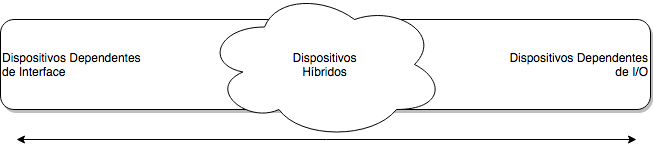
\includegraphics[width=0.9\textwidth]{img/rt-gradiente.png}
			%\vspace{-10pt}
			\caption{Classificação de sistemas \wearables. De um extremo existe os dispositivos dependentes de interfaces de usuário e do outro os dependentes de entrada e saída de sinais enquanto entre eles, a gama de combinações possíveis. Fonte: Adaptado de \citep{Amorim2017}.}
			\label{fig:classification}
		\end{figure}

		De um lado desta gama de dispositivos existem os \emph{dispositivos dependentes de interfaces de usuário} que possuem alta dependência com operações interfaces gráficas, provendo respostas sobre as interações do usuário.
      Esses dispositivos focam principalmente em tarefas para renderização em \textit{displays} como por exemplo equipamentos de realidade virtual e aumentada para implementação de objetos tridimensionais.
      %
		De outro lado, existem os \emph{dispositivos dependentes de entrada e saída de sinais}. Esses dispositivos atuam principalmente com o estímulo por algum dado oriundo de outro dispositivo ou do ambiente assim entregue à nuvem respeitando restrições de tempo real.
      Isso se da pela utilização de sensores acoplados ao dispositivo que podem exigir uma boa vazão de dados e pequena latência como são os monitores de atividade remota, situação na qual cria-se o ambiente perfeito para o termo conhecido por IoT (do inglês \textit{Internet of Things}).

		Entre dispositivos dependentes de interfaces de usuário e de entrada e saída de sinais existe os híbridos. São dispositivos que utilizam recursos de ambos os extremos citados.
      Dispositivos como \textit{smartwatches} e \textit{fitness trackers} são exemplos de tais dispositivos híbridos no qual possuem restrições de equalização à prioridade dada pelo dispositivo para ambas as operações de interface e sinais.

		A separação dos conceitos computação \wearable\ e IoT ainda não estão claros segundo a bibliografia.
      Sistemas operacionais de propósito específico para ambientes \wearable\ são comumente focado em um único tipo de seguimento de produto como os \textit{smartwatches}, sendo que proporciona aos desenvolvedores um meio para sua aplicação final além de entregar um produto de alta qualidade.
      Também, atualmente, não existe nenhum sistema que satisfaça todos os requisitos apresentados \citep{Amorim2017}.

		Já \citet{Jozwiak2017} caracteriza um sistema \wearable\ como um sistema \textit{cyber}-físico\footnote{Sendo \textit{cyber-} uma combinação dos termos `computador', `rede de computadores' ou `realidade virtual' com um segundo termo, no caso o `físico' oriundo de circuitos.} móvel autônomo.
      São sistemas que podem ter mobilidade inerente ou poder ser transportado para outro sistema, industrial ou natural (incluindo humanos), sendo autônomos em termos de funcionalidade.
      Podem ser utilizados para aplicações de consumidores (computação móvel), extensões ou reposições de capacidades humanas, sistemas sociais (\textit{health-care} inteligente), automotivo, industrial (monitoramento) e aplicações comerciais como realidade aumentada para informações turísticas.
		Eles representam uma grande parte da heterogeneidade de sistemas embarcados, cobrindo muitos campos e tipos de aplicações que vão desde um dispositivo inteligente integrado à roupa, focado no campo de computação \textit{mobile} pessoal, até indústrias como dispositivos de segurança. % \citep{Jozwiak2017}.
      Esses dispositivos podem também trabalhar de forma colaborativa com \textit{smartphones}, redes e outros sistemas criando um sistema mais complexo.

		Segundo \citet{VanLaerhoven2002}, a distribuição de elementos computacionais, como sensores, em objetos mundanos em nosso cotidiano se adéqua à pesquisa denominada por computação ubíqua.
      Isso implica também que computação \wearable\ também não foge deste arcabouço, uma vez que superfícies de roupas são uma plataforma de suporte ideal para uma grande quantidade de sensores (desde que sejam miniaturizados para que eles não obstruam o usuário).
		Essa restrição de tamanho geralmente significa que a própria qualidade do equipamento também está comprometida, o que leva ao conceito de muitos atuadores e sensores simplistas.

		Sendo sistemas \wearables\ uma subclasse de sistemas embutidos, estão sujeitos à várias restrições de \design, sendo elas performance em multi-nós, gasto energético consciente e alta flexibilidade \citep{Plessl2003}:

     \begin{description}
       	\item [Performance de multi-nós:] Requer uma performance base fixa para tarefas que não mostram altas demandas computacionais nem restrições de tempo rigorosa.
            Sistemas \wearables\ executam rajadas de tarefas de computação intensiva que consideram restrições de tempo-real.
            Não realizando as tarefas, o sistema torna-se inaplicável.

		   \item [Gasto energético consciente:] É essencial em sistema deve-se manter ativo e funcional num certo período de tempo.
            O \design\ do gasto de energia conduz inúmeros desafios como gerenciamento computacional energético eficiente e energização dinâmica.

            Diferenciando os termos de baixo custo de energia e eficiência energético, o consumo de energia é mensurado pela divisão da dissipação energética pelo tempo mensurado.
            %
            A eficiência energética relaciona o total de energia necessário para computar uma tarefa específica sendo o desafio a construção de um \design\ na qual possui-se alta eficiência energética para um dado conjunto de tarefas.
            O procedimento dinâmico de energização consiste na tarefa de associar determinada tarefa para o componente mais eficiente (energeticamente falando) disponível e forçar todos os outros não utilizados pelo sistema a serem postos em modo de economia de energia ou desligá-los quando apropriadamente.

   		\item [Flexibilidade:] Quando menciona-se sobre alta flexibilidade, é considerado o fato de que o dispositivo será utilizado em situações altamente dinâmicas.
            Isso fica claro na necessidade na qual os requisitos de aplicação variam de acordo com as escolhas do usuário, mas também com o contexto e local utilizado.
            Outro, é no fato de que o usuário troca de roupas constantemente e com isso os dispositivos devem ter a capacidade de serem acoplados e removidos, neste caso.
            Isso além de critérios como confiabilidade, disponibilidade e fatores dependentes de sua forma como volume e peso.
     \end{description}

		Dessa forma, pode-se estabelecer que os requisitos flexíveis em um sistema \wearable\ demanda um sistema de computação programável de propósito geral, enquanto os requisitos de alta performance e consumo de energia consciente demandam um sistema computacional especializado.
      Assim, como meio para solução desses problemas, \citeauthor{Plessl2003} utilizaram-se de um \hardware\ reconfigurável para incorporar ao sistema.
      O trabalho exibe um sistema \wearables\ compreendendo de um processador de até médio porte em termos de processamento e módulos reconfiguráveis.
		A utilização de \hardware\ reconfigurável nos permite alcançar alto processamento com maior eficiência energética em relação à processadores para tarefas de computação intensiva em tempo real.
